\chapter{SynthFairy, FairPrism y mas allá...}
\label{cap:fairPrism}

\section{Experimental Validation} \label{sec:experimental_eval}

\definecolor{Gray}{gray}{0.9}
\definecolor{Gray2}{gray}{0.95}
\newcolumntype{g}{>{\columncolor{Gray}}c}
\newcolumntype{h}{>{\columncolor{Gray2}}c}

In order to evaluate the viability of our approach we have  extended the model checker {\Prism}~\cite{DBLP:conf/cav/KwiatkowskaN0S20,DBLP:conf/cav/KwiatkowskaNP11} with an operator to compute the expected rewards for stochastic games that stop under fairness. The prototype also allows one to check whether a game is stopping under fairness.
%implemented a prototype tool named \textsf{SynthFairy} (available at \cite{SynthFairy})
%and run it on two different sets of examples. %\footnote{Available at \cite{SynthFairy}}. 
The tool takes as input a model describing the game in {\Prism} notation and returns as output 
the optimal expected total reward  for a given  initial state as well as the synthesized optimal controller strategy (under fairness assumptions). 
%The input models are specified using a language resembling {\Prism} notation \cite{DBLP:conf/cav/KwiatkowskaNP11}. 
The experimental  evaluation shows that our approach can cope with non-trivial  case studies. For computing these values we set a relative error of at most $\varepsilon = 10^{-6}$.


%We have considered variations of two examples:
%For the model presented in Sec.~\ref{sec:mot_example}, the expected total reward when $\verb"P"=0.1$ and $\verb"Q"=0$ is $5.55$. Moreover, 
%the non-trivial part of the synthesized strategy is illustrated with the black arrows in Fig.~\ref{fig:robot_game_grid}.

\paragraph{Roborta vs. the Fair Light.}  Table~\ref{table:resultsRobot} shows the results of the example introduced in Sec.~\ref{sec:mot_example} 
for multiple configurations. 
We considered three variants of the case study: version A (the light does not fail), version B (the light can only fail when trying to signal a green light), and version C (the light can fail when trying to signal any kind of light). 
We assumed that, when Roborta  fails,  she cannot move (this is beneficial to Roborta since she can re-collect the reward);
when the light fails, the robot can freely move into any allowed direction. 
The grid configuration (movement restrictions and rewards) are randomly generated.  For each setting, Table~\ref{table:resultsRobot} describes the results for three different scenarios generated starting at different seeds.  For the grid configuration shown in Sec.~\ref{sec:mot_example} with  parameters $P=0.1$ and $Q=0$, the tool derived the optimal strategy depicted in Fig.~\ref{fig:robot_game_grid} and reports an expected total reward of $5.55$. 

%We explain Table~\ref{table:resultsRobot} with an example.  Take the case of the grid $A \mid {60{\times}8} \mid \text{seed } 1$, with the robot fault probability being $0.1$, the optimal expected total reward is $26.66$ and the number of decisions made by the robot when both players play optimally is $2$.  We consider a decision as a choice resolution introduced when the yellow light is on on a cell without movement restrictions or if the light is off. We use this number to give us an idea that resolutions are not trivial, and to hint a different resolution for closely related instances.
%Indeed, notice that for the case mentioned above, when the fault probability is set to $0.9$ (instead of $0.1$), the number of decisions changes to $0$. 
%This suggests that the strategy of the environment for lower fault probabilities was not worth it anymore, thereby it finds a better strategy. 


% Figure follows ------------------
\begin{wrapfigure}[11]{r}{48mm}
%\vspace{-10mm}
\vspace{-11mm}
%\fontsize{6.6}{6.6}\selectfont\ttfamily
\centering
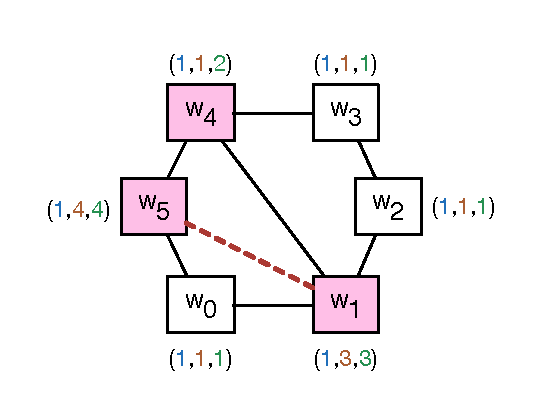
\includegraphics[scale=0.60]{Figs/uav.eps}\hspace{1.5em}\mbox{}
\vspace{-10mm}
\caption{UAV Network for ISR missions adapted from \cite{DBLP:conf/iccps/FengWHT15}} \label{fig:uav_game_map}
%\caption{A robot game on a $4 \times 4$ grid starting on location (0,0). Each location has an assigned positive reward. The sideway movement restrictions are depicted as white arrows on the bottom-right of each location. The best strategy for the robot when the light is yellow is shown in black arrows on the top-right of the locations without movement restrictions. The path taken by the robot to achieve the goal is highlighted in yellow} \label{fig:robot_game_grid}
\end{wrapfigure}
%
\paragraph{Autonomous UAV vs. Human Operator.} We adapted the case study analyzed in  \cite{DBLP:conf/iccps/FengWHT15}. A remotely controlled Unmanned Aerial Vehicle (UAV) is used to perform intelligence, surveillance, and reconnaissance (ISR) missions over a road network. The UAV performs piloting functions autonomously (selecting a path to fly between \emph{waypoints}). The human operator (environment) controls the onboard sensor to capture imagery at a waypoint as well as the piloting functions on certain waypoints (called checkpoints). Note that an operator can continuously try to get a better image by making the UAV loiter around a certain waypoint, this may lead to an unfair behavior.
%We assign rewards to a successful capture of an unvisited waypoint.
Each successful capture from an unvisited waypoint grants a reward.
% 
Fig.~\ref{fig:uav_game_map} shows an example of road network consisting of six surveillance waypoints labeled $w_0,w_2,...,w_5$, the edges represent connecting paths, a red-dashed line means that the path is dangerous enough to make the UAV stop working with probability $1$, while on any other path, this probability is $S$. Checkpoints are depicted as pink nodes, therein the operator can still delegate the piloting task to the UAV with probability $D$. Each node is annotated with three possible rewards. For instance,  for $S=0.3$ and $D=0.5$ and the leftmost reward values in each triple, the synthesized strategy for the UAV tries to follow the optimal circuit $w_0,w_1,w_2,w_3,w_4,w_5$. While for  the middle and  rightmost reward values, the optimal circuits to follow are $w_0,w_5,w_0,w_1,w_2,w_3,w_4$ and $w_0,w_5,w_4,w_1,w_2,w_3$, respectively.   Table~\ref{table:resultsUAV} shows the results obtained for  this game for several randomly generated road networks.

Tables~\ref{table:resultsRobot} and~\ref{table:resultsUAV} do not report the time taken to compute the results,   but in all cases the output was computed in less than 400 seconds.All the experiments were run on a MacBook Air with Intel Core i5 at 1.3 GHz and 4 Gb of RAM. %The tool and case studies are available in the tool repository.
%\remarkPRD{Poner aqu'i un comentario sobre el desempe\~no de la herramienta respecto del tiempo}

\begin{table}[tp]
  \centering\noindent%
  %\vspace{-0.5cm}
  \caption{Results for Roborta vs. Light Game.  First column describes the grid size.  Second column indicates  the fault probability for the robot ($P$) and light ($Q$). 
  The other columns describe the size of the model, the expected total reward for the optimal strategy, and the number of iterations performed, respectively,
  for three different randomly generated grid configurations.}
  \label{table:resultsRobot}
  %\vspace{-0.8cm}
  \scalebox{0.9}{
    \begin{tabular}{|c|c|c|c|c|c|g|h|c|g|h|c|}
      \hline
      \multirow{2}{*}{Version} & \multicolumn{2}{c|}{Fault prob.} & \multicolumn{3}{c|}{Size (States/Transitions)} & \multicolumn{3}{c|}{Opt.\ Expect.\ Total Rew.} & \multicolumn{3}{c|}{Iterations}\\ \hhline{|~|-|-|-|-|-|-|-|-|-|-|-|}
      & $P$ & $Q$ &  \cellcolor{white}s.\ 1 & \cellcolor{white}s.\ 2 & \cellcolor{white}s.\ 3 & \cellcolor{white}\makebox[3.4em][c]{s.\ 1} & \cellcolor{white}\makebox[3.4em][c]{s.\ 2} & \cellcolor{white}\makebox[3.4em][c]{s.\ 3} & \cellcolor{white}\makebox[1.8em][c]{s.\ 1} & \cellcolor{white}\makebox[1.8em][c]{s.\ 2} & \cellcolor{white}\makebox[1.8em][c]{s.\ 3}  \\  
      \hline
       \multirow{2}{3em}{\centering $A$ \\ $60{\times}8$}
       & $0.1$ & $-$ & \multirow{2}{*}{\centering $\displaystyle \begin{array}{c} \text{st. }1448 \\ \text{tr. }3220 \end{array}$} & \multirow{2}{*}{\centering $\displaystyle \begin{array}{c} \text{st. }1418 \\ \text{tr. }3112 \end{array}$}  & \multirow{2}{*}{\centering $\displaystyle \begin{array}{c} \text{st. }1421 \\ \text{tr. }3132 \end{array}$}  & $26.66$ & $31.11$ & $27.77$ & $711$ & $681$ & $252$\\ \hhline{|~|-|-|~|~|~|-|-|-|-|-|-|}
       & $0.5$ & $-$ & & & & $48$ & $56$ & $50$ & $2253$ & $2225$ & $475$\\ \hline

       \multirow{2}{3em}{\centering $A$ \\ $120{\times}16$}
       & $0.1$ & $-$ & \multirow{2}{*}{\centering $\displaystyle \begin{array}{c} \text{st. }5686 \\ \text{tr. }12586 \end{array}$} & \multirow{2}{*}{\centering $\displaystyle \begin{array}{c} \text{st. }5716 \\ \text{tr. }12658 \end{array}$}  & \multirow{2}{*}{\centering $\displaystyle \begin{array}{c} \text{st. }5716 \\ \text{tr. }12722 \end{array}$}  & $62.22$ & $55.55$ & $48.88$ & $687$ & $700$ & $685$ \\ \hhline{|~|-|-|~|~|~|-|-|-|-|-|-|}
       & $0.5$ & $-$ & & & & $112$ & $100$ & $88$ & $2231$ & $2265$ & $2229$ \\ \hline

       \multirow{4}{3em}{\centering $B$ \\ $60{\times}8$}
       & \multirow{2}{*}{$0.1$} & $0.1$ & \multirow{4}{*}{\centering $\displaystyle \begin{array}{c} \text{st. }1928 \\ \text{tr. }5952 \end{array}$} & \multirow{4}{*}{\centering $\displaystyle \begin{array}{c} \text{st. }1888 \\ \text{tr. }5746 \end{array}$}  & \multirow{4}{*}{\centering $\displaystyle \begin{array}{c} \text{st. }1892 \\ \text{tr. }5785 \end{array}$}  & $42.6$ & $44.59$ & $42.23$ & $479$ & $335$ & $388$ \\ \hhline{|~|~|-|~|~|~|-|-|-|-|-|-|}
       & & $0.5$ & & & & $130.14$ & $127.7$ & $136.22$ & $772$ & $689$ & $824$ \\ \hhline{|~|-|-|~|~|~|-|-|-|-|-|-|}
       & \multirow{2}{*}{$0.5$} & $0.1$ & & & & $76.68$ & $80.26$ & $76.02$ & $873$ & $764$ & $909$ \\ \hhline{|~|~|-|~|~|~|-|-|-|-|-|-|}
       & & $0.5$ & & & & $234.26$ & $229.87$ & $245.21$ & $1263$ & $1139$ & $1341$ \\ \hline

       \multirow{4}{3em}{\centering $B$ \\ $120{\times}16$}
       & \multirow{2}{*}{$0.1$} & $0.1$ & \multirow{4}{*}{\centering $\displaystyle \begin{array}{c} \text{st. }7576 \\ \text{tr. }23266 \end{array}$} & \multirow{4}{*}{\centering $\displaystyle \begin{array}{c} \text{st. }7616 \\ \text{tr. }23400 \end{array}$}  & \multirow{4}{*}{\centering $\displaystyle \begin{array}{c} \text{st. }7616 \\ \text{tr. }23528 \end{array}$}  & $91.19$ & $87.27$ & $80.07$ & $538$ & $544$ & $616$ \\ \hhline{|~|~|-|~|~|~|-|-|-|-|-|-|}
       & & $0.5$ & & & & $281.83$ & $281.48$ & $265.33$ & $1076$ & $1118$ & $1252$\\ \hhline{|~|-|-|~|~|~|-|-|-|-|-|-|}
       & \multirow{2}{*}{$0.5$} & $0.1$ & & & & $164.15$ & $157.1$ & $144.13$ & $1147$ & $1223$ & $1373$ \\ \hhline{|~|~|-|~|~|~|-|-|-|-|-|-|}
       & & $0.5$ & & & & $507.30$ & $506.67$ & $477.6$ & $1850$ & $1865$ & $2088$ \\ \hline

       \multirow{4}{3em}{\centering $C$ \\ $60{\times}8$}
       & \multirow{2}{*}{$0.1$} & $0.1$ & \multirow{4}{*}{\centering $\displaystyle \begin{array}{c} \text{st. }1928 \\ \text{tr. }6432 \end{array}$} & \multirow{4}{*}{\centering $\displaystyle \begin{array}{c} \text{st. }1888 \\ \text{tr. }6216 \end{array}$}  & \multirow{4}{*}{\centering $\displaystyle \begin{array}{c} \text{st. }1892 \\ \text{tr. }6256 \end{array}$}  & $46.32$ & $47.07$ & $44.87$ & $379$ & $336$ & $390$ \\ \hhline{|~|~|-|~|~|~|-|-|-|-|-|-|}
       & & $0.5$ & & & & $143.35$ & $146.41$ & $153.98$ & $742$ & $658$ & $774$ \\ \hhline{|~|-|-|~|~|~|-|-|-|-|-|-|}
       & \multirow{2}{*}{$0.5$} & $0.1$ & & & & $83.37$ & $84.73$ & $80.77$ & $879$ & $769$ & $914$ \\ \hhline{|~|~|-|~|~|~|-|-|-|-|-|-|}
       & & $0.5$ & & & & $258.04$ & $263.53$ & $277.17$ & $1202$ & $1076$ & $1246$ \\ \hline

       \multirow{4}{3em}{\centering $C$ \\ $120{\times}16$}
       & \multirow{2}{*}{$0.1$} & $0.1$ & \multirow{4}{*}{\centering $\displaystyle \begin{array}{c} \text{st. }7576 \\ \text{tr. }25156 \end{array}$} & \multirow{4}{*}{\centering $\displaystyle \begin{array}{c} \text{st. }7616 \\ \text{tr. }25300 \end{array}$}  & \multirow{4}{*}{\centering $\displaystyle \begin{array}{c} \text{st. }7616 \\ \text{tr. }25428 \end{array}$}  & $98.25$ & $93.74$ & $88.33$ & $533$ & $544$ & $606$ \\ \hhline{|~|~|-|~|~|~|-|-|-|-|-|-|}
       & & $0.5$ & & & & $321.18$ & $317.61$ & $311.62$ & $1002$ & $1068$ & $1188$ \\ \hhline{|~|-|-|~|~|~|-|-|-|-|-|-|}
       & \multirow{2}{*}{$0.5$} & $0.1$ & & & & $176.85$ & $168.73$ & $158.99$ & $1147$ & $1227$ & $1365$\\ \hhline{|~|~|-|~|~|~|-|-|-|-|-|-|}
       & & $0.5$ & & & & $578.13$ & $571.71$ & $560.92$ & $1700$ & $1760$ & $1956$ \\ 

      \hline
    \end{tabular}
  }
  %\vspace{-0.8cm}
\end{table}

\begin{table}[tp]
  \centering\noindent%
  %\vspace{-0.5cm}
  \caption{Results for the UAV vs. Operator Game. First column describes the number of waypoints used.  Second column indicates probability of delegation ($D$), and the probability that the UAV stops working ($S$). 
  The other columns show the size of the model, the expected total reward for the optimal strategy, and the number of iterations performed, respectively, for three different randomly generated roadmap configurations.}
  \label{table:resultsUAV}
  %\vspace{-0.8cm}
  \scalebox{0.9}{
    \begin{tabular}{|c|c|c|c|c|c|g|h|c|g|h|c|}
      \hline
      \multirow{2}{*}{Version} & \multicolumn{2}{c|}{Prob.} & \multicolumn{3}{c|}{Size(States/Transitions)} & \multicolumn{3}{c|}{Opt.\ Expect.\ Total Rew.} & \multicolumn{3}{c|}{Iterations} \\ \hhline{|~|-|-|-|-|-|-|-|-|-|-|-|}
      & $D$ & $S$ &  \cellcolor{white}s.\ 1 & \cellcolor{white}s.\ 2 & \cellcolor{white}s.\ 3 & \cellcolor{white}\makebox[3.4em][c]{s.\ 1} & \cellcolor{white}\makebox[3.4em][c]{s.\ 2} & \cellcolor{white}\makebox[3.4em][c]{s.\ 3} & \cellcolor{white}\makebox[1.8em][c]{s.\ 1} & \cellcolor{white}\makebox[1.8em][c]{s.\ 2} & \cellcolor{white}\makebox[1.8em][c]{s.\ 3} \\  
      \hline
       \multirow{4}{3em}{\centering UAV \\ $6w.$}
       & \multirow{2}{*}{$0.1$} & $0.05$ & \multirow{4}{*}{\centering $\displaystyle \begin{array}{c} \text{st. }213 \\ \text{tr. }504 \end{array}$} & \multirow{4}{*}{\centering $\displaystyle \begin{array}{c} \text{st. }508 \\ \text{tr. }1368 \end{array}$} & \multirow{4}{*}{\centering $\displaystyle \begin{array}{c} \text{st. }136 \\ \text{tr. }312 \end{array}$} & $16.72$ & $12.47$ & $13.14$ & $142$ & $248$ & $22$ \\ \hhline{|~|~|-|~|~|~|-|-|-|-|-|-|}
       & & $0.1$ & & & & $15.73$ & $11.15$ & $12.63$ & $73$ & $188$ & $22$ \\ \hhline{|~|-|-|~|~|~|-|-|-|-|-|-|}
       & \multirow{2}{*}{$0.5$} & $0.05$ & & & & $20.49$ & $12.77$ & $17.05$ & $103$ & $133$ & $22$ \\ \hhline{|~|~|-|~|~|~|-|-|-|-|-|-|}
       & & $0.1$ & & & & $18.87$ & $11.67$ & $15.95$ & $55$ & $70$ & $22$ \\ \hline

       \multirow{4}{3em}{\centering UAV \\ $8w.$}
       & \multirow{2}{*}{$0.1$} & $0.05$ & \multirow{4}{*}{\centering $\displaystyle \begin{array}{c} \text{st. }2177 \\ \text{tr. }5959 \end{array}$} & \multirow{4}{*}{\centering $\displaystyle \begin{array}{c} \text{st. }3591 \\ \text{tr. }9991 \end{array}$} & \multirow{4}{*}{\centering $\displaystyle \begin{array}{c} \text{st. }1426 \\ \text{tr. }3604 \end{array}$} & $17.88$ & $40.59$ & $24.6$ & $407$ & $332$ & $779$ \\ \hhline{|~|~|-|~|~|~|-|-|-|-|-|-|}
       & & $0.1$ & & & & $17.11$ & $34.3$ & $21.48$ & $280$ & $233$ & $437$ \\ \hhline{|~|-|-|~|~|~|-|-|-|-|-|-|}
       & \multirow{2}{*}{$0.5$} & $0.05$ & & & & $26$ & $42.21$ & $30.87$ & $128$ & $214$ & $257$ \\ \hhline{|~|~|-|~|~|~|-|-|-|-|-|-|}
       & & $0.1$ & & & & $23.44$ & $36.08$ & $24.72$ & $116$ & $113$ & $194$ \\ \hline 

       \multirow{4}{3em}{\centering UAV \\ $10w.$}
       & \multirow{2}{*}{$0.1$} & $0.05$ & \multirow{4}{*}{\centering $\displaystyle \begin{array}{c} \text{st. }6631 \\ \text{tr. }17306 \end{array}$} & \multirow{4}{*}{\centering $\displaystyle \begin{array}{c} \text{st. }5072 \\ \text{tr. }13052 \end{array}$} & \multirow{4}{*}{\centering $\displaystyle \begin{array}{c} \text{st. }8272 \\ \text{tr. }24376 \end{array}$} & $39.76$ & $28.7$ & $19.76$ & $256$ & $377$ & $356$ \\ \hhline{|~|~|-|~|~|~|-|-|-|-|-|-|} 
       & & $0.1$ & & & & $35.43$ & $23.36$ & $16.2$ & $136$ & $260$ & $154$ \\ \hhline{|~|-|-|~|~|~|-|-|-|-|-|-|}
       & \multirow{2}{*}{$0.5$} & $0.05$ & & & & $42.13$ & $30.77$ & $24.56$ & $250$ & $247$ & $292$ \\ \hhline{|~|~|-|~|~|~|-|-|-|-|-|-|}
       & & $0.1$ & & & & $37.11$ & $26.08$ & $19.27$ & $130$ & $134$ & $151$\\ \hline

      \hline
    \end{tabular}
  }
  %\vspace{-0.8cm}
\end{table}












































%TABLAS FAIRYGAMES CON TIEMPOS
\iffalse
\begin{table}[t]
  \centering\noindent%
  %\vspace{-0.5cm}
  \caption{Results for Roborta vs. Light Game.  First column describes the grid size.  Second column indicates  the fault probability for the robot ($P$) and light ($Q$). 
  The other columns describe the size of the model, the expected total reward for the optimal strategy, and the computation  time in seconds, respectively,
  for three different randomly generated grid configurations.}
  \label{table:resultsRobot}
  %\vspace{-0.8cm}
  \scalebox{0.9}{
    \begin{tabular}{|c|c|c|c|c|c|g|h|c|g|h|c|g|h|c|}
      \hline
      \multirow{2}{*}{Version} & \multicolumn{2}{c|}{Fault prob.} & \multicolumn{3}{c|}{Size (States/Transitions)} & \multicolumn{3}{c|}{Opt.\ Expect.\ Total Rew.} & \multicolumn{3}{c|}{N.Iter.} & \multicolumn{3}{c|}{Time (in sec.)}\\ \hhline{|~|-|-|-|-|-|-|-|-|-|-|-|-|-|-|}
      & $P$ & $Q$ &  \cellcolor{white}s.\ 1 & \cellcolor{white}s.\ 2 & \cellcolor{white}s.\ 3 & \cellcolor{white}\makebox[3.4em][c]{s.\ 1} & \cellcolor{white}\makebox[3.4em][c]{s.\ 2} & \cellcolor{white}\makebox[3.4em][c]{s.\ 3} & \cellcolor{white}\makebox[1.8em][c]{s.\ 1} & \cellcolor{white}\makebox[1.8em][c]{s.\ 2} & \cellcolor{white}\makebox[1.8em][c]{s.\ 3} & \cellcolor{white}\makebox[1.8em][c]{s.\ 1} & \cellcolor{white}\makebox[1.8em][c]{s.\ 2} & \cellcolor{white}\makebox[1.8em][c]{s.\ 3} \\  
      \hline
       \multirow{2}{3em}{\centering $A$ \\ $60{\times}8$}
       & $0.1$ & $-$ & \multirow{2}{*}{\centering $\displaystyle \begin{array}{c} \text{st. }1448 \\ \text{tr. }3220 \end{array}$} & \multirow{2}{*}{\centering $\displaystyle \begin{array}{c} \text{st. }1418 \\ \text{tr. }3112 \end{array}$}  & \multirow{2}{*}{\centering $\displaystyle \begin{array}{c} \text{st. }1421 \\ \text{tr. }3132 \end{array}$}  & $26.66$ & $31.11$ & $27.77$ & $711$ & $681$ & $252$ & $3$ & $3$ & $3$\\ \hhline{|~|-|-|~|~|~|-|-|-|-|-|-|-|-|-|}
       & $0.5$ & $-$ & & & & $48$ & $56$ & $50$ & $2253$ & $2225$ & $475$ & $7$ & $6$ & $2$\\ \hline

       \multirow{2}{3em}{\centering $A$ \\ $120{\times}16$}
       & $0.1$ & $-$ & \multirow{2}{*}{\centering $\displaystyle \begin{array}{c} \text{st. }5686 \\ \text{tr. }12586 \end{array}$} & \multirow{2}{*}{\centering $\displaystyle \begin{array}{c} \text{st. }5716 \\ \text{tr. }12658 \end{array}$}  & \multirow{2}{*}{\centering $\displaystyle \begin{array}{c} \text{st. }5716 \\ \text{tr. }12722 \end{array}$}  & $62.22$ & $55.55$ & $48.88$ & $687$ & $700$ & $685$ & $147$ & $152$ & $150$\\ \hhline{|~|-|-|~|~|~|-|-|-|-|-|-|-|-|-|}
       & $0.5$ & $-$ & & & & $112$ & $100$ & $88$ & $2231$ & $2265$ & $2229$ & $135$ & $147$ & $176$\\ \hline

       \multirow{4}{3em}{\centering $B$ \\ $60{\times}8$}
       & \multirow{2}{*}{$0.1$} & $0.1$ & \multirow{4}{*}{\centering $\displaystyle \begin{array}{c} \text{st. }1928 \\ \text{tr. }5952 \end{array}$} & \multirow{4}{*}{\centering $\displaystyle \begin{array}{c} \text{st. }1888 \\ \text{tr. }5746 \end{array}$}  & \multirow{4}{*}{\centering $\displaystyle \begin{array}{c} \text{st. }1892 \\ \text{tr. }5785 \end{array}$}  & $42.6$ & $44.59$ & $42.23$ & $479$ & $335$ & $388$ & $4$ & $5$ & $5$\\ \hhline{|~|~|-|~|~|~|-|-|-|-|-|-|-|-|-|}
       & & $0.5$ & & & & $130.14$ & $127.7$ & $136.22$ & $772$ & $689$ & $824$ & $5$ & $5$ & $5$\\ \hhline{|~|-|-|~|~|~|-|-|-|-|-|-|-|-|-|}
       & \multirow{2}{*}{$0.5$} & $0.1$ & & & & $76.68$ & $80.26$ & $76.02$ & $873$ & $764$ & $909$ & $4$ & $3$ & $4$\\ \hhline{|~|~|-|~|~|~|-|-|-|-|-|-|-|-|-|}
       & & $0.5$ & & & & $234.26$ & $229.87$ & $245.21$ & $1263$ & $1139$ & $1341$ & $5$ & $9$ & $9$\\ \hline

       \multirow{4}{3em}{\centering $B$ \\ $120{\times}16$}
       & \multirow{2}{*}{$0.1$} & $0.1$ & \multirow{4}{*}{\centering $\displaystyle \begin{array}{c} \text{st. }7576 \\ \text{tr. }23266 \end{array}$} & \multirow{4}{*}{\centering $\displaystyle \begin{array}{c} \text{st. }7616 \\ \text{tr. }23400 \end{array}$}  & \multirow{4}{*}{\centering $\displaystyle \begin{array}{c} \text{st. }7616 \\ \text{tr. }23528 \end{array}$}  & $91.19$ & $87.27$ & $80.07$ & $538$ & $544$ & $616$ & $275$ & $285$ & $241$\\ \hhline{|~|~|-|~|~|~|-|-|-|-|-|-|}
       & & $0.5$ & & & & $281.83$ & $281.48$ & $265.33$ & $1076$ & $1118$ & $1252$ & $300$ & $336$ & $279$\\ \hhline{|~|-|-|~|~|~|-|-|-|-|-|-|-|-|-|}
       & \multirow{2}{*}{$0.5$} & $0.1$ & & & & $164.15$ & $157.1$ & $144.13$ & $1147$ & $1223$ & $1373$ & $169$ & $238$ & $313$\\ \hhline{|~|~|-|~|~|~|-|-|-|-|-|-|-|-|-|}
       & & $0.5$ & & & & $507.30$ & $506.67$ & $477.6$ & $1850$ & $1865$ & $2088$ & $327$ & $354$ & $313$\\ \hline

       \multirow{4}{3em}{\centering $C$ \\ $60{\times}8$}
       & \multirow{2}{*}{$0.1$} & $0.1$ & \multirow{4}{*}{\centering $\displaystyle \begin{array}{c} \text{st. }1928 \\ \text{tr. }6432 \end{array}$} & \multirow{4}{*}{\centering $\displaystyle \begin{array}{c} \text{st. }1888 \\ \text{tr. }6216 \end{array}$}  & \multirow{4}{*}{\centering $\displaystyle \begin{array}{c} \text{st. }1892 \\ \text{tr. }6256 \end{array}$}  & $46.32$ & $47.07$ & $44.87$ & $379$ & $336$ & $390$ & $6$ & $4$ & $5$\\ \hhline{|~|~|-|~|~|~|-|-|-|-|-|-|-|-|-|}
       & & $0.5$ & & & & $143.35$ & $146.41$ & $153.98$ & $742$ & $658$ & $774$ & $6$ & $5$ & $5$\\ \hhline{|~|-|-|~|~|~|-|-|-|-|-|-|-|-|-|}
       & \multirow{2}{*}{$0.5$} & $0.1$ & & & & $83.37$ & $84.73$ & $80.77$ & $879$ & $769$ & $914$ & $6$ & $3$ & $4$\\ \hhline{|~|~|-|~|~|~|-|-|-|-|-|-|-|-|-|}
       & & $0.5$ & & & & $258.04$ & $263.53$ & $277.17$ & $1202$ & $1076$ & $1246$ & $7$ & $4$ & $9$\\ \hline

       \multirow{4}{3em}{\centering $C$ \\ $120{\times}16$}
       & \multirow{2}{*}{$0.1$} & $0.1$ & \multirow{4}{*}{\centering $\displaystyle \begin{array}{c} \text{st. }7576 \\ \text{tr. }25156 \end{array}$} & \multirow{4}{*}{\centering $\displaystyle \begin{array}{c} \text{st. }7616 \\ \text{tr. }25300 \end{array}$}  & \multirow{4}{*}{\centering $\displaystyle \begin{array}{c} \text{st. }7616 \\ \text{tr. }25428 \end{array}$}  & $98.25$ & $93.74$ & $88.33$ & $533$ & $544$ & $606$ & $257$ & $267$ & $236$\\ \hhline{|~|~|-|~|~|~|-|-|-|-|-|-|-|-|-|}
       & & $0.5$ & & & & $321.18$ & $317.61$ & $311.62$ & $1002$ & $1068$ & $1188$ & $291$ & $274$ & $264$\\ \hhline{|~|-|-|~|~|~|-|-|-|-|-|-|-|-|-|}
       & \multirow{2}{*}{$0.5$} & $0.1$ & & & & $176.85$ & $168.73$ & $158.99$ & $1147$ & $1227$ & $1365$ & $246$ & $213$ & $228$\\ \hhline{|~|~|-|~|~|~|-|-|-|-|-|-|-|-|-|}
       & & $0.5$ & & & & $578.13$ & $571.71$ & $560.92$ & $1700$ & $1760$ & $1956$ & $339$ & $291$ & $292$\\ 

      \hline
    \end{tabular}
  }
  %\vspace{-0.8cm}
\end{table}

\begin{table}[t]
  \centering\noindent%
  %\vspace{-0.5cm}
  \caption{Results for the UAV vs. Operator Game. First column describes the number of waypoints used.  Second column indicates probability of delegation ($D$), and the probability that the UAV stops working ($S$). 
  The other columns show the size of the model, the expected total reward for the optimal strategy, and the computation time in seconds, respectively, for three different randomly generated roadmap configurations.}
  \label{table:resultsUAV}
  %\vspace{-0.8cm}
  \scalebox{0.9}{
    \begin{tabular}{|c|c|c|c|c|c|g|h|c|g|h|c|g|h|c|}
      \hline
      \multirow{2}{*}{Version} & \multicolumn{2}{c|}{Prob.} & \multicolumn{3}{c|}{Size(States/Transitions)} & \multicolumn{3}{c|}{Opt.\ Expect.\ Total Rew.} & \multicolumn{3}{c|}{N.Iter.} & \multicolumn{3}{c|}{Time (in sec.)} \\ \hhline{|~|-|-|-|-|-|-|-|-|-|-|-|-|-|-|}
      & $D$ & $S$ &  \cellcolor{white}s.\ 1 & \cellcolor{white}s.\ 2 & \cellcolor{white}s.\ 3 & \cellcolor{white}\makebox[3.4em][c]{s.\ 1} & \cellcolor{white}\makebox[3.4em][c]{s.\ 2} & \cellcolor{white}\makebox[3.4em][c]{s.\ 3} & \cellcolor{white}\makebox[1.8em][c]{s.\ 1} & \cellcolor{white}\makebox[1.8em][c]{s.\ 2} & \cellcolor{white}\makebox[1.8em][c]{s.\ 3} & \cellcolor{white}\makebox[1.8em][c]{s.\ 1} & \cellcolor{white}\makebox[1.8em][c]{s.\ 2} & \cellcolor{white}\makebox[1.8em][c]{s.\ 3}\\  
      \hline
       \multirow{4}{3em}{\centering UAV \\ $6w.$}
       & \multirow{2}{*}{$0.1$} & $0.05$ & \multirow{4}{*}{\centering $\displaystyle \begin{array}{c} \text{st. }213 \\ \text{tr. }504 \end{array}$} & \multirow{4}{*}{\centering $\displaystyle \begin{array}{c} \text{st. }508 \\ \text{tr. }1368 \end{array}$} & \multirow{4}{*}{\centering $\displaystyle \begin{array}{c} \text{st. }136 \\ \text{tr. }312 \end{array}$} & $16.72$ & $12.47$ & $13.14$ & $142$ & $248$ & $22$ & $0$ & $0$ & $0$\\ \hhline{|~|~|-|~|~|~|-|-|-|-|-|-|-|-|-|}
       & & $0.1$ & & & & $15.73$ & $11.15$ & $12.63$ & $73$ & $188$ & $22$ & $0$ & $0$ & $0$\\ \hhline{|~|-|-|~|~|~|-|-|-|-|-|-|-|-|-|}
       & \multirow{2}{*}{$0.5$} & $0.05$ & & & & $20.49$ & $12.77$ & $17.05$ & $103$ & $133$ & $22$ & $0$ & $0$ & $0$\\ \hhline{|~|~|-|~|~|~|-|-|-|-|-|-|-|-|-|}
       & & $0.1$ & & & & $18.87$ & $11.67$ & $15.95$ & $55$ & $70$ & $22$ & $0$ & $0$ & $0$\\ \hline

       \multirow{4}{3em}{\centering UAV \\ $8w.$}
       & \multirow{2}{*}{$0.1$} & $0.05$ & \multirow{4}{*}{\centering $\displaystyle \begin{array}{c} \text{st. }2177 \\ \text{tr. }5959 \end{array}$} & \multirow{4}{*}{\centering $\displaystyle \begin{array}{c} \text{st. }3591 \\ \text{tr. }9991 \end{array}$} & \multirow{4}{*}{\centering $\displaystyle \begin{array}{c} \text{st. }1426 \\ \text{tr. }3604 \end{array}$} & $17.88$ & $40.59$ & $24.6$ & $407$ & $332$ & $779$ & $8$ & $29$ & $4$\\ \hhline{|~|~|-|~|~|~|-|-|-|-|-|-|-|-|-|}
       & & $0.1$ & & & & $17.11$ & $34.3$ & $21.48$ & $280$ & $233$ & $437$ & $3$ & $17$ & $3$\\ \hhline{|~|-|-|~|~|~|-|-|-|-|-|-|-|-|-|}
       & \multirow{2}{*}{$0.5$} & $0.05$ & & & & $26$ & $42.21$ & $30.87$ & $128$ & $214$ & $257$ & $6$ & $26$ & $2$\\ \hhline{|~|~|-|~|~|~|-|-|-|-|-|-|-|-|-|}
       & & $0.1$ & & & & $23.44$ & $36.08$ & $24.72$ & $116$ & $113$ & $194$ & $3$ & $16$ & $2$\\ \hline 

       \multirow{4}{3em}{\centering UAV \\ $10w.$}
       & \multirow{2}{*}{$0.1$} & $0.05$ & \multirow{4}{*}{\centering $\displaystyle \begin{array}{c} \text{st. }6631 \\ \text{tr. }17306 \end{array}$} & \multirow{4}{*}{\centering $\displaystyle \begin{array}{c} \text{st. }5072 \\ \text{tr. }13052 \end{array}$} & \multirow{4}{*}{\centering $\displaystyle \begin{array}{c} \text{st. }8272 \\ \text{tr. }24376 \end{array}$} & $39.76$ & $28.7$ & $19.76$ & $256$ & $377$ & $356$ & $133$ & $62$ & $264$\\ \hhline{|~|~|-|~|~|~|-|-|-|-|-|-|-|-|-|} 
       & & $0.1$ & & & & $35.43$ & $23.36$ & $16.2$ & $136$ & $260$ & $154$ & $62$ & $43$ & $119$\\ \hhline{|~|-|-|~|~|~|-|-|-|-|-|-|-|-|-|}
       & \multirow{2}{*}{$0.5$} & $0.05$ & & & & $42.13$ & $30.77$ & $24.56$ & $250$ & $247$ & $292$ & $126$ & $63$ & $229$\\ \hhline{|~|~|-|~|~|~|-|-|-|-|-|-|-|-|-|}
       & & $0.1$ & & & & $37.11$ & $26.08$ & $19.27$ & $130$ & $134$ & $151$ & $59$ & $40$ & $97$\\ \hline

      \hline
    \end{tabular}
  }
  %\vspace{-0.8cm}
\end{table}
\fi


%TABLAS SYNTHFAIRY
\iffalse
\begin{table}[t]
  \centering\noindent%
  %\vspace{-0.5cm}
  \caption{Results for Roborta vs. Light Game.  First column describes the grid size.  Second column indicates  the fault probability for the robot ($P$) and light ($Q$). 
  The other columns describe the size of the model, the expected total reward for the optimal strategy, and the computation  time in seconds, respectively,
  for three different randomly generated grid configurations.}
  \label{table:resultsRobot}
  %\vspace{-0.8cm}
  \scalebox{0.9}{
    \begin{tabular}{|c|c|c|c|c|c|g|h|c|g|h|c|}
      \hline
      \multirow{2}{*}{Version} & \multicolumn{2}{c|}{Fault prob.} & \multicolumn{3}{c|}{Size (States/Transitions)} & \multicolumn{3}{c|}{Opt.\ Expect.\ Total Rew.} & \multicolumn{3}{c|}{Time (in sec.)} \\ \hhline{|~|-|-|-|-|-|-|-|-|-|-|-|}
      & $P$ & $Q$ &  \cellcolor{white}s.\ 1 & \cellcolor{white}s.\ 2 & \cellcolor{white}s.\ 3 & \cellcolor{white}\makebox[3.4em][c]{s.\ 1} & \cellcolor{white}\makebox[3.4em][c]{s.\ 2} & \cellcolor{white}\makebox[3.4em][c]{s.\ 3} & \cellcolor{white}\makebox[1.8em][c]{s.\ 1} & \cellcolor{white}\makebox[1.8em][c]{s.\ 2} & \cellcolor{white}\makebox[1.8em][c]{s.\ 3} \\  
      \hline
       \multirow{2}{3em}{\centering $A$ \\ $60{\times}8$}
       & $0.1$ & $-$ & \multirow{2}{*}{\centering $\displaystyle \begin{array}{c} \text{st. }2614 \\ \text{tr. }4418 \end{array}$} & \multirow{2}{*}{\centering $\displaystyle \begin{array}{c} \text{st. }2540 \\ \text{tr. }4266 \end{array}$}  & \multirow{2}{*}{\centering $\displaystyle \begin{array}{c} \text{st. }2552 \\ \text{tr. }4295 \end{array}$}  & $26.66$ & $31.11$ & $27.77$ & $10$ & $9$ & $12$\\ \hhline{|~|-|-|~|~|~|-|-|-|-|-|-|}
       & $0.5$ & $-$ & & & & $48$ & $56$ & $50$ & $14$ & $16$ & $12$\\ \hline

       \multirow{2}{3em}{\centering $A$ \\ $120{\times}16$}
       & $0.1$ & $-$ & \multirow{2}{*}{\centering $\displaystyle \begin{array}{c} \text{st. }10161 \\ \text{tr. }17125 \end{array}$} & \multirow{2}{*}{\centering $\displaystyle \begin{array}{c} \text{st. }10217 \\ \text{tr. }17223 \end{array}$}  & \multirow{2}{*}{\centering $\displaystyle \begin{array}{c} \text{st. }10249 \\ \text{tr. }17319 \end{array}$}  & $62.22$ & $55.55$ & $48.88$ & $99$ & $116$ & $96$\\ \hhline{|~|-|-|~|~|~|-|-|-|-|-|-|}
       & $0.5$ & $-$ & & & & $112$ & $100$ & $88$ & $133$ & $149$ & $137$\\ \hline

       \multirow{4}{3em}{\centering $B$ \\ $60{\times}8$}
       & \multirow{2}{*}{$0.1$} & $0.1$ & \multirow{4}{*}{\centering $\displaystyle \begin{array}{c} \text{st. }4724 \\ \text{tr. }8788 \end{array}$} & \multirow{4}{*}{\centering $\displaystyle \begin{array}{c} \text{st. }4586 \\ \text{tr. }8484 \end{array}$}  & \multirow{4}{*}{\centering $\displaystyle \begin{array}{c} \text{st. }4609 \\ \text{tr. }8542 \end{array}$}  & $42.6$ & $44.59$ & $42.23$ & $20$ & $24$ & $21$\\ \hhline{|~|~|-|~|~|~|-|-|-|-|-|-|}
       & & $0.5$ & & & & $130.14$ & $127.7$ & $136.22$ & $32$ & $33$ & $30$\\ \hhline{|~|-|-|~|~|~|-|-|-|-|-|-|}
       & \multirow{2}{*}{$0.5$} & $0.1$ & & & & $76.68$ & $80.26$ & $76.02$ & $32$ & $31$ & $32$\\ \hhline{|~|~|-|~|~|~|-|-|-|-|-|-|}
       & & $0.5$ & & & & $234.26$ & $229.87$ & $245.21$ & $53$ & $50$ & $56$\\ \hline

       \multirow{4}{3em}{\centering $B$ \\ $120{\times}16$}
       & \multirow{2}{*}{$0.1$} & $0.1$ & \multirow{4}{*}{\centering $\displaystyle \begin{array}{c} \text{st. }18384 \\ \text{tr. }34154 \end{array}$} & \multirow{4}{*}{\centering $\displaystyle \begin{array}{c} \text{st. }18486 \\ \text{tr. }34350 \end{array}$}  & \multirow{4}{*}{\centering $\displaystyle \begin{array}{c} \text{st. }18550 \\ \text{tr. }34542 \end{array}$}  & $91.19$ & $87.27$ & $80.07$ & $260$ & $250$ & $277$\\ \hhline{|~|~|-|~|~|~|-|-|-|-|-|-|}
       & & $0.5$ & & & & $281.83$ & $281.48$ & $265.33$ & $375$ & $366$ & $359$\\ \hhline{|~|-|-|~|~|~|-|-|-|-|-|-|}
       & \multirow{2}{*}{$0.5$} & $0.1$ & & & & $164.15$ & $157.1$ & $144.13$ & $389$ & $378$ & $376$\\ \hhline{|~|~|-|~|~|~|-|-|-|-|-|-|}
       & & $0.5$ & & & & $507.30$ & $506.67$ & $477.6$ & $555$ & $553$ & $535$\\ \hline

       \multirow{4}{3em}{\centering $C$ \\ $60{\times}8$}
       & \multirow{2}{*}{$0.1$} & $0.1$ & \multirow{4}{*}{\centering $\displaystyle \begin{array}{c} \text{st. }5212 \\ \text{tr. }9764 \end{array}$} & \multirow{4}{*}{\centering $\displaystyle \begin{array}{c} \text{st. }5064 \\ \text{tr. }9440 \end{array}$}  & \multirow{4}{*}{\centering $\displaystyle \begin{array}{c} \text{st. }5088 \\ \text{tr. }9500 \end{array}$}  & $46.32$ & $47.07$ & $44.87$ & $23$ & $22$ & $23$\\ \hhline{|~|~|-|~|~|~|-|-|-|-|-|-|}
       & & $0.5$ & & & & $143.35$ & $146.41$ & $153.98$ & $34$ & $32$ & $34$\\ \hhline{|~|-|-|~|~|~|-|-|-|-|-|-|}
       & \multirow{2}{*}{$0.5$} & $0.1$ & & & & $83.37$ & $84.73$ & $80.77$ & $36$ & $34$ & $34$\\ \hhline{|~|~|-|~|~|~|-|-|-|-|-|-|}
       & & $0.5$ & & & & $258.04$ & $263.53$ & $277.17$ & $54$ & $51$ & $52$\\ \hline

       \multirow{4}{3em}{\centering $C$ \\ $120{\times}16$}
       & \multirow{2}{*}{$0.1$} & $0.1$ & \multirow{4}{*}{\centering $\displaystyle \begin{array}{c} \text{st. }20290 \\ \text{tr. }37966 \end{array}$} & \multirow{4}{*}{\centering $\displaystyle \begin{array}{c} \text{st. }20402 \\ \text{tr. }38182 \end{array}$}  & \multirow{4}{*}{\centering $\displaystyle \begin{array}{c} \text{st. }20466 \\ \text{tr. }38374 \end{array}$}  & $98.25$ & $93.74$ & $88.33$ & $297$ & $297$ & $331$\\ \hhline{|~|~|-|~|~|~|-|-|-|-|-|-|}
       & & $0.5$ & & & & $321.18$ & $317.61$ & $311.62$ & $405$ & $403$ & $496$\\ \hhline{|~|-|-|~|~|~|-|-|-|-|-|-|}
       & \multirow{2}{*}{$0.5$} & $0.1$ & & & & $176.85$ & $168.73$ & $158.99$ & $440$ & $426$ & $527$\\ \hhline{|~|~|-|~|~|~|-|-|-|-|-|-|}
       & & $0.5$ & & & & $578.13$ & $571.71$ & $560.92$ & $606$ & $640$ & $723$\\ 

      \hline
    \end{tabular}
  }
  %\vspace{-0.8cm}
\end{table}

\begin{table}[t]
  \centering\noindent%
  %\vspace{-0.5cm}
  \caption{Results for the UAV vs. Operator Game. First column describes the number of waypoints used.  Second column indicates probability of delegation ($D$), and the probability that the UAV stops working ($S$). 
  The other columns show the size of the model, the expected total reward for the optimal strategy, and the computation time in seconds, respectively, for three different randomly generated roadmap configurations.}
  \label{table:resultsUAV}
  %\vspace{-0.8cm}
  \scalebox{0.9}{
    \begin{tabular}{|c|c|c|c|c|c|g|h|c|g|h|c|}
      \hline
      \multirow{2}{*}{Version} & \multicolumn{2}{c|}{Prob.} & \multicolumn{3}{c|}{Size(States/Transitions)} & \multicolumn{3}{c|}{Opt.\ Expect.\ Total Rew.} & \multicolumn{3}{c|}{Time (in sec.)} \\ \hhline{|~|-|-|-|-|-|-|-|-|-|-|-|}
      & $D$ & $S$ &  \cellcolor{white}s.\ 1 & \cellcolor{white}s.\ 2 & \cellcolor{white}s.\ 3 & \cellcolor{white}\makebox[3.4em][c]{s.\ 1} & \cellcolor{white}\makebox[3.4em][c]{s.\ 2} & \cellcolor{white}\makebox[3.4em][c]{s.\ 3} & \cellcolor{white}\makebox[1.8em][c]{s.\ 1} & \cellcolor{white}\makebox[1.8em][c]{s.\ 2} & \cellcolor{white}\makebox[1.8em][c]{s.\ 3} \\  
      \hline
       \multirow{4}{3em}{\centering UAV \\ $6w.$}
       & \multirow{2}{*}{$0.1$} & $0.05$ & \multirow{4}{*}{\centering $\displaystyle \begin{array}{c} \text{st. }501 \\ \text{tr. }857 \end{array}$} & \multirow{4}{*}{\centering $\displaystyle \begin{array}{c} \text{st. }1148 \\ \text{tr. }2166 \end{array}$} & \multirow{4}{*}{\centering $\displaystyle \begin{array}{c} \text{st. }302 \\ \text{tr. }508 \end{array}$} & $16.72$ & $12.47$ & $13.14$ & $8$ & $25$ & $1$\\ \hhline{|~|~|-|~|~|~|-|-|-|-|-|-|}
       & & $0.1$ & & & & $15.73$ & $11.15$ & $12.63$ & $5$ & $14$ & $2$\\ \hhline{|~|-|-|~|~|~|-|-|-|-|-|-|}
       & \multirow{2}{*}{$0.5$} & $0.05$ & & & & $20.49$ & $12.77$ & $17.05$ & $7$ & $22$ & $3$\\ \hhline{|~|~|-|~|~|~|-|-|-|-|-|-|}
       & & $0.1$ & & & & $18.8$ & $11.67$ & $15.95$ & $7$ & $13$ & $2$\\ \hline

       \multirow{4}{3em}{\centering UAV \\ $8w.$}
       & \multirow{2}{*}{$0.1$} & $0.05$ & \multirow{4}{*}{\centering $\displaystyle \begin{array}{c} \text{st. }5335 \\ \text{tr. }9734 \end{array}$} & \multirow{4}{*}{\centering $\displaystyle \begin{array}{c} \text{st. }8289 \\ \text{tr. }15642 \end{array}$} & \multirow{4}{*}{\centering $\displaystyle \begin{array}{c} \text{st. }3167 \\ \text{tr. }5723 \end{array}$} & $17.88$ & $40.59$ & $24.6$ & $47$ & $183$ & $51$\\ \hhline{|~|~|-|~|~|~|-|-|-|-|-|-|}
       & & $0.1$ & & & & $17.11$ & $34.3$ & $21.48$ & $63$ & $128$ & $31$\\ \hhline{|~|-|-|~|~|~|-|-|-|-|-|-|}
       & \multirow{2}{*}{$0.5$} & $0.05$ & & & & $26$ & $42.21$ & $30.87$ & $67$ & $209$ & $41$\\ \hhline{|~|~|-|~|~|~|-|-|-|-|-|-|}
       & & $0.1$ & & & & $23.44$ & $36.08$ & $24.72$ & $51$ & $114$ & $27$\\ \hline

       \multirow{4}{3em}{\centering UAV \\ $10w.$}
       & \multirow{2}{*}{$0.1$} & $0.05$ & \multirow{4}{*}{\centering $\displaystyle \begin{array}{c} \text{st. }15775 \\ \text{tr. }28257 \end{array}$} & \multirow{4}{*}{\centering $\displaystyle \begin{array}{c} \text{st. }11212 \\ \text{tr. }20624 \end{array}$} & \multirow{4}{*}{\centering $\displaystyle \begin{array}{c} \text{st. }21153 \\ \text{tr. }39348 \end{array}$} & $39.76$ & $28.7$ & $19.76$ & $659$ & $656$ & $892$\\ \hhline{|~|~|-|~|~|~|-|-|-|-|-|-|}
       & & $0.1$ & & & & $35.43$ & $23.36$ & $16.2$ & $389$ & $261$ & $586$\\ \hhline{|~|-|-|~|~|~|-|-|-|-|-|-|}
       & \multirow{2}{*}{$0.5$} & $0.05$ & & & & $42.13$ & $30.77$ & $24.56$ & $644$ & $421$ & $891$\\ \hhline{|~|~|-|~|~|~|-|-|-|-|-|-|}
       & & $0.1$ & & & & $37.11$ & $26.08$ & $19.27$ & $412$ & $261$ & $592$\\ \hline

      \hline
    \end{tabular}
  }
  %\vspace{-0.8cm}
\end{table}
\fi
